\section{Metrics}
\label{sec:background:metrics}

Within the field of text detection, various evaluation protocols exist. For an extensive survey of these protocols, see \citep{Wolf:2006gv,Ye:2014bs}. Throughout our survey, we note the standard the evaluation scheme for text extraction first proposed for use in image processing in the \glsx{icdar} competitions \citep{Lucas:2003iw, Lucas:2005bq, Shahab:2011hq, Karatzas:2013by, Karatzas:2015tj}. This scheme was designed to be easy to understand and compute, reward text extraction useful for natural scenes, and heavily punish trivial solutions. The intention behind these metrics were to develop a measure of `robustness' a text extraction pipeline can achieve. 

In the \gls{icdar} competitions, two are used: the initial \gls{icdar} 2003 evaluation protocol proposed by \citet{Lucas:2003iw}, and, more recently, the \textit{DetEval} evaluation protocol \citep{Shivakumara:2011dn} (based on \citep{Wolf:2006gv}), as used in the \gls{icdar} 2011 and 2013 robust reading competitions. The simplicity and continued wide use of the \gls{icdar} 2003 for text localisation evaluation is chosen over the \textit{DetEval} approach, especially as it complements our use case.

\subsection{Precision and Recall}
\label{sec:background:metrics:precision_and_recall}

Generally in information retrieval, the precision ($p$) and recall ($r$) metrics are used, first defined in the six evaluation criteria for information retrieval systems by \citet{Cleverdon:1966vd}. Precision refers to the proportion of relevant matches actually retrieved in the results, while recall refers to the proportion of relevant matches retrieved in total relevant instances. We use recall and precision metrics to assess the \textit{effectiveness} of an information retrieval system \citep{Rijsbergen:1979dw}.

In the context of image processing, systems that over-estimate are punished with a low precision score, while systems that under-estimate are punished with a low recall score \citep{Lucas:2003iw}. Therefore, precision is the number of correct candidates ($c$) divided by the number of total estimates found ($E$):
\begin{equation*}
  p = \frac{c}{\lvert\;E\;\rvert}
\end{equation*}

And recall is defined as the number of correct estimates divided by the total number of ground-set truth targets ($T$):
\begin{equation*}
  r = \frac{c}{\lvert\;T\;\rvert}
\end{equation*}

However, it is not realistic for a given text extraction pipeline to \textit{exactly} agree with the rectangle bounds manually tagged by a human. \citet{Lucas:2003iw} first proposed changes to these calculations to better suit their usage in the context of information extraction from within images. They adopt a more flexible notion of what a `match' is. They define a new match measure, the match area $m_{a}$, between two rectangles (i.e., the ground truth and the system's detected candidate) as the area of intersection of both rectangles divided by the minimum bounding box containing both rectangles (i.e., the union of both) \citep{Lucas:2003iw, Lucas:2005bq, Lucas:2005hl}. This metric is otherwise commonly referred to as the \gls{iou} \citep{Karatzas:2015tj,Lin:2014vma,Jaderberg:2016wj}. Using $a(r)$ to denote the area of the rectangle, we can represent this as:
\begin{equation*}
  m_{a}(r_{1}, r_{2}) = \frac{a(r_{1} \cap r_{2})}{a(r_{1} \cup r_{2})}
\end{equation*}

This allows for a match value of one when the candidate is identical to the ground truth, and zero where the candidate has no intersection at all to the ground truth. Therefore, the best match, $m(r,\,R)$, of a rectangle $r$ in a set of rectangles $R$ is:
\begin{equation*}
  m(r,\,R) = \mathrm{max}~\{~m_{a}(r,\,r')~|~r' \in R~\}
\end{equation*}

Lastly, we can redefine the recall and precision metrics to be more forgiving in the image extraction context:
\begin{align*}
  p' &= \frac{\sum\,_{r_{e}\;\in\;E}~m(r_{e},\,T)}{\lvert\;E\;\rvert}\\\\
  r' &= \frac{\sum\,_{r_{t}\;\in\;T}~m(r_{t},\,E)}{\lvert\;T\;\rvert}
\end{align*}

One issue with the calculation is that it assumes a rectangular bounding box. Words of non-rectangular nature, such as curved or rhomboidal text, are not well-represented.

\subsection{The \fscore}
\label{sec:background:metrics:fscore}

A common metric used when developing text extraction pipelines is the \fscore, a single measure of quality that combines both precision and recall values. We are able to compute this metric using the standard measure across many studies, as contrasted in Table~\ref{tab:background:metrics:survey}.

The \fscore{} algorithm is given in the context of image processing in \citet{Lucas:2003iw}. Relative weights controlled by an $\alpha$ value of 0.5 give equal weight to both precision and recall metrics:
\begin{equation*}
  f = \frac{1}{\frac{\alpha}{p'} + \frac{1-\alpha}{r'}}
\end{equation*}

As \citet{Chen:2011ul} report, even when all text is correctly localised, it is likely that the \fscore{} will vary between 0.8--1.0. This is because $E$ boundaries are unlikely to match \textit{exactly} with the manually labelled $T$ boundaries. An illustration of this is phenomena is shown in Figure~\ref{fig:background:metrics:ye2005_overlapping}.

\begin{figure}[p]
  \centering
  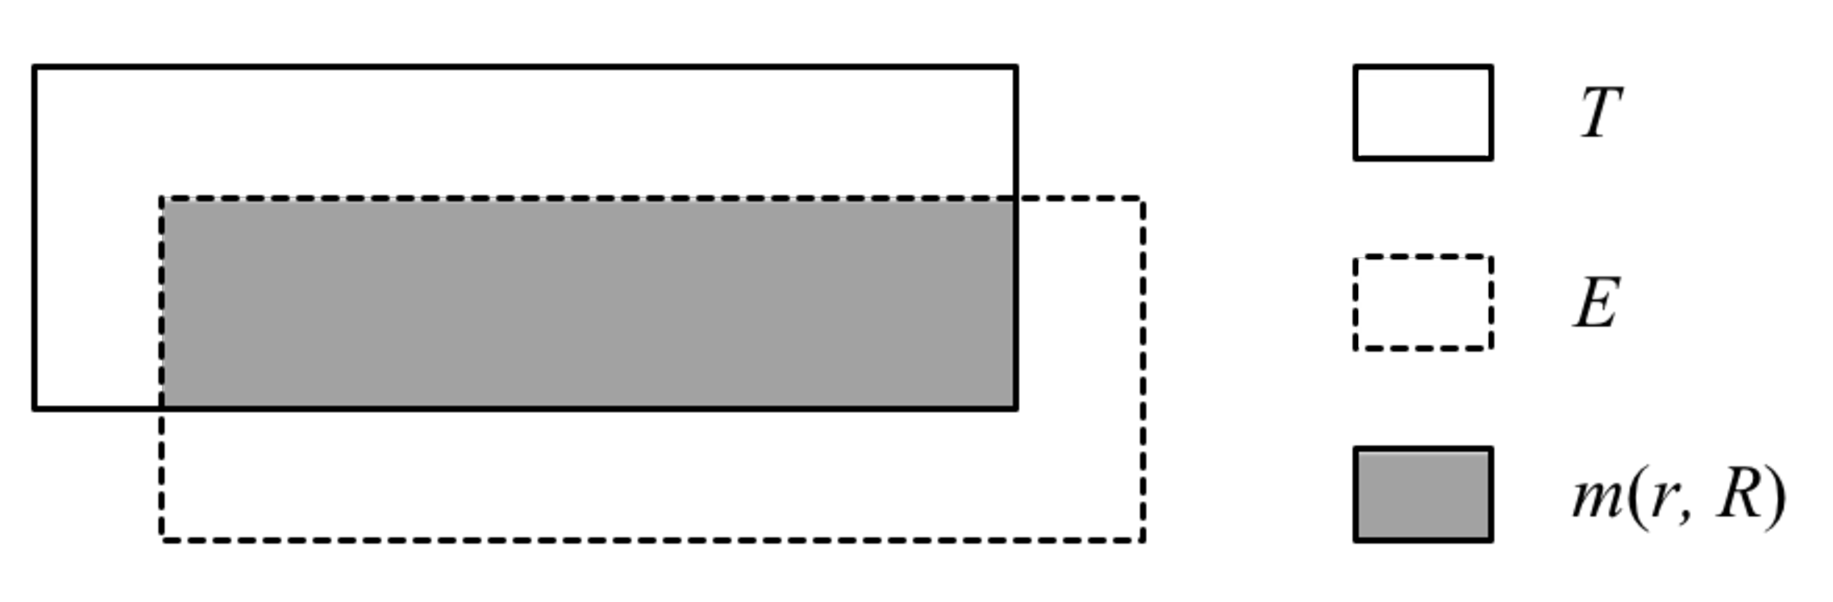
\includegraphics[width=0.65\textwidth]{images/background/ye2005_overlapping}
  \caption[Overlapping areas of ground truth and estimated targets]{Overlapping areas of the ground truth targets, $T$, the estimated target boundaries $E$ and the best match $m(r,\;R)$. (Adapted from \citep{Ye:2005wu}.)}
  \label{fig:background:metrics:ye2005_overlapping}
\end{figure}

\begin{table}[]
  \newcommand{\ccbased}[0]{\textit{\gls{cc}-based}:}
  \newcommand{\lgbased}[0]{\textit{Learning-based}:}
  \newcommand{\ns}[0]{N/S}
  \newcommand{\twods}[2]{\makecell[l]{#1\\#2}}
  \centering
  \caption[Survey of text extraction literature]{\centering A survey of text extraction literature, separated into \gls{cc}- and learning-based detection methods.}
  \label{tab:background:metrics:survey}
  \tablefit{
    \begin{tabular}{@{}llp{0.45\textwidth}p{0.15\textwidth}lllcll@{}}
      \toprule
        \multirow{2}{*}{\bfseries Ref.} &
        \multirow{2}{*}{\bfseries Year} &
        \multicolumn{2}{c}{\bfseries Scientific Background} &
        \multirow{2}{*}{\bfseries Precision} &
        \multirow{2}{*}{\bfseries Recall} &
        \multirow{2}{*}{\bfseries \fscore} &
        \multirow{2}{*}{\bfseries Dataset(s)} &
        \multicolumn{2}{c}{\bfseries Performance} 
      \\
        \cmidrule(lr){3-4}
        \cmidrule(l){9-10} &
        &
        \textbf{Detection} &
        \textbf{Recognition} &
        &
        &
        &
        &
        \textbf{Platform} &
        \textbf{Time (s)}
      \\
      \midrule
        \citep{Benami:2012jf} &
        \citeyear{Benami:2012jf} &
        \ccbased{} \gls{swt}; Canny-Edges; Binary Conversion; Geometric Filtering; \gls{cc}-Alignment &
        OCR (Tesseract) &
        0.65 &
        0.62 &
        0.63 &
        N/A &
        \ns{} &
        \ns{}
      \\
        \citep{Chen:2011ul} &
        \citeyear{Chen:2011ul} &
        \ccbased{} Canny-Edges; \gls{mser}; \gls{swt}, Geometric, Template Matching &
        OCR (\ns{}\textsuperscript{$\dagger$}) &
        0.73 &
        0.60 &
        0.66 &
        \citep{Lucas:2003iw,Lucas:2005bq} & 
        2.5 GHz &
        0.20
      \\ 
        \citep{Li:2012wd} &
        \citeyear{Li:2012wd} &
        \ccbased{} \gls{mser}; geometric and \gls{swt} filters; skeletal distance mapping &
        \ns{} &
        \twods{0.59 \citep{Lucas:2003iw}}{0.59 \citep{Shahab:2011hq}} &
        \twods{0.59 \citep{Lucas:2003iw}}{0.62 \citep{Shahab:2011hq}} &
        \twods{0.59 \citep{Lucas:2003iw}}{0.61 \citep{Shahab:2011hq}} &
        \citep{Lucas:2005bq,Shahab:2011hq} & 
        \ns{} &
        \ns{}
      \\
        \citep{Zhang:2011cl} &
        \citeyear{Zhang:2011cl} &
        \ccbased{} character detection with \gls{hog} and \gls{swt}; link energies via spacial relationships between characters &
        \ns{} &
        0.73 &
        0.62 &
        0.67 &
        \citep{Lucas:2003iw} &
        \ns{} &
        \ns{}
      \\
        \citep{Shivakumara:2011dn} &
        \citeyear{Shivakumara:2011dn} &
        \ccbased{} Fourier-Laplacian Filtering; clustering based on maximum distance via K-Means; skeletal distance mapping &
        \ns{} &
        \twods{0.76 \citep{Lucas:2003iw}}{0.81 \citep{Hua:2004vf}} &
        \twods{0.86 \citep{Lucas:2003iw}}{0.93 \citep{Hua:2004vf}} &
        \twods{0.81 \citep{Lucas:2003iw}}{0.87 \citep{Hua:2004vf}} &
        \citep{Lucas:2003iw, Hua:2004vf} &
        2.0 GHz &
        7.80
      \\
        \citep{Epshtein:2010tj} &
        \citeyear{Epshtein:2010tj} &
        \ccbased{} Canny-Edges; \gls{swt}; Modified \gls{cc} algorithm; Geometric Filtering &
        OCR (\ns{}) &
        0.73 &
        0.60 &
        0.66 &
        \citep{Lucas:2003iw, Lucas:2005bq} &
        \ns{} &
        0.94
      \\
        \citep{Zhang:2010wa} &
        \citeyear{Zhang:2010wa} &
        \ccbased{} Canny-Edges; \gls{hog}; geometric filtering; graph spectrum &
        \ns{} &
        0.67 &
        0.46 &
        0.55 &
        \citep{Lucas:2003iw} &
        \ns{} &
        \ns{}
      \\
      \midrule
      \midrule
        \citep{Ye:2005wu} &
        \citeyear{Ye:2005wu} &
        \lgbased{} \gls{svm} to reject non-text; wavelet movement; \gls{hog}; \gls{ocr} filtering &
        \ns{} &
        \ns{} &
        0.97 &
        \ns{} &
        \citep{Hua:2004vf} &
        1.6 GHz &
        8.30
      \\
        \citep{Pan:2010cj} &
        \citeyear{Pan:2010cj} &
        \lgbased{} Waldboost Classifier; \gls{hog}; \gls{lbp}; Gabor Wavelets &
        \ns{} &
        0.56 &
        0.70 &
        0.68 &
        \citep{Lucas:2003iw} &
        3.4 GHz &
        0.37
      \\
        \citep{Gllavata:2004vq} &
        \citeyear{Gllavata:2004vq} &
        \lgbased{} Wavelet transformation; feature estimation; pixel-block classification &
        \ns{} &
        0.87 &
        0.90 &
        0.88 &
        \citep{Hua:2001un} &
        \ns{} &
        \ns{}
      \\
        \citep{Hanif:2009tm} &
        \citeyear{Hanif:2009tm} &
        \lgbased{} Mean Difference, Standard Deviation and \gls{hog} features; AdaBoost and CAdaBoost classifiers; \gls{nn}-baed localiser &
        \ns{} &
        0.25 &
        0.35 &
        0.35 &
        \citep{Lucas:2003iw} &
        2.2 GHz &
        \ns{}
      \\
      \bottomrule
    \end{tabular}
  }
  \\
  \bigskip
  {\footnotesize \textsuperscript{$\dagger$}Not Specified}
\end{table}